\section*{Problema 5}

\textbf{Sea c una cierta cadena binaria de longitud 100. Se quiere verificar si proviene de una muestra $Bern(0.5)(=H_0)$. Para eso se calcula el número de cambios. Un cambio es un 1 seguido por un 0 o un 0 seguido por un 1 en la cadena.}

\begin{enumerate}
	\item  Calcula T el número de cambios en una cadena usando una sola linea de código en R.

	      Para realizar el calculo del número de cambios se hizo en base a la diferencia del i-esimo elemento y el i+1. En el caso en que este sea 00 o 11, la diferencia es 0. Por ende el 0 representa que no existe un cambio. En cambio 01 y 10, produce una diferencia de -1 y 1 respectivamente. Por ende, al tomar el valor absoluto, 1 representa que existio un cambio en la cadena. Al realizar la suma de estas diferencias se obtiene el número de cambios totales en la cadena. Por lo tanto, el código para conseguir el número de cambios en una cadena es el siguiente:

	      \begin{verbatim}
								change <- sum(abs(diff(chain)))
			\end{verbatim}

	\item Usando muchas simulaciones de cadenas bajo $H_0$ , estima y visualiza la distribución de T.

	      La distribución usando un espacio de 1000 bootstrap se representa en la figura \ref{fig:problema5_distribution}.

	      \begin{figure}[H]
		      \centering
		      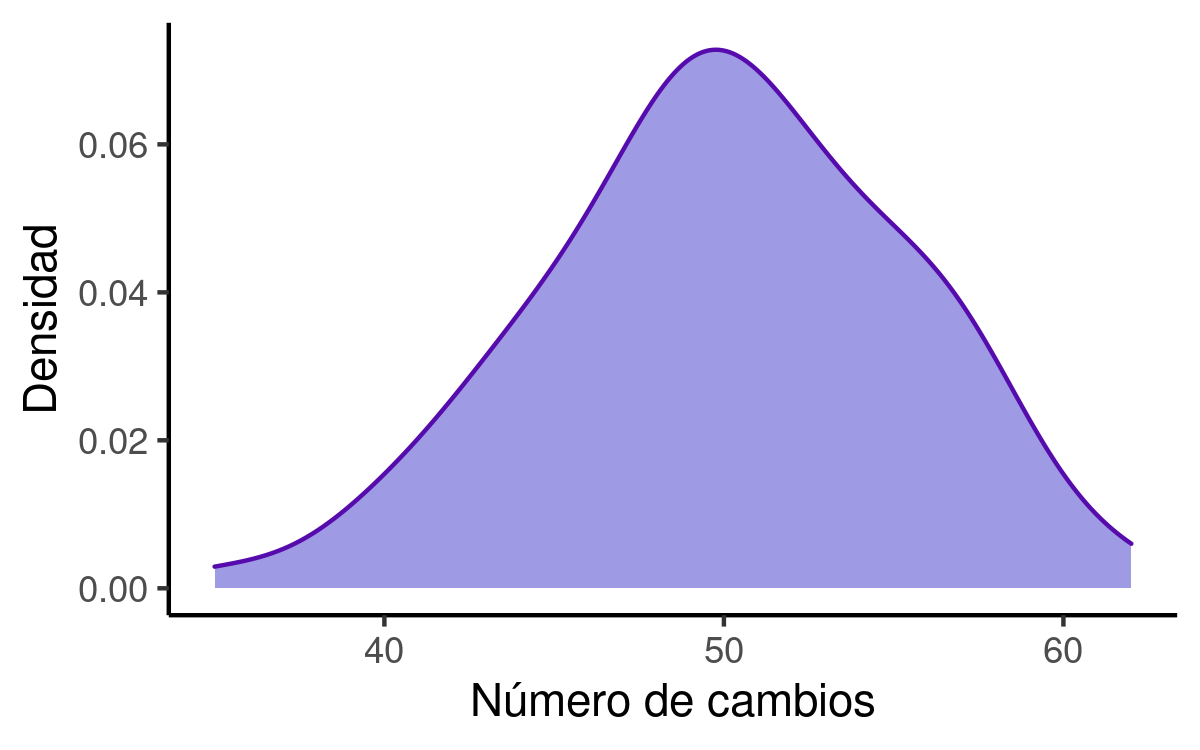
\includegraphics[width=14cm]{Graphics/problema05.png}
		      \caption{Distribución del número de cambios en una cadena de 100 elementos.}
		      \label{fig:problema5_distribution}
	      \end{figure}
	\item Calcula el valor de p para $H_0$ si T=42.

	      Se tiene que la media y varianza de la cadena binaria es $50.5000$ y $5.4542$ respectivamente. Por lo que calculando el valor de p con el comando \script{pt(mu-42)/(sigma/sqrt(n))}, se obtiene que es $9.384e-290$.


\end{enumerate}
